\graphicspath{{./chapitres/chapitre7/figures/}}
\setcounter{mtc}{7}
\chapter{Sprint Cinq: Expérimentation en Data Mining}
\minitoc
\newpage
\section*{Introduction}
Notre projet est en réalité un projet à long terme qui est divisé sur plusieurs parties. Ce que nous avons réalisé jusqu'ici est une première partie du projet.\newline
Concernant la suite du projet, c'est un nouveau mini projet pour mener une analyse avancée sur les transactions (prédiction,  classification, clustering ,etc).\newline
Dans ce chapitre nous allons mettre en place un petit exemple sous forme d'une expérimentation pour avoir une vision plus claire sur les prochaines étapes dans le futur.
\section{Sprint Backlog}
\subsection{Histoires \`a r\'ealiser}
Le tableau \ref{tab:sprint5backlog} d\'ecrit les histoires du backlog de ce sprint.

\begin{longtable}[!ht]{|l|l|c|}
\hline
{\textbf{Feature}} & {\textbf{Technical Story}} & {\textbf{Story Points}}\\
\hline
\multirow{2}{3cm}{\textbf{ Une formation Python et Flask}} & R\&D Python   & 3 \\
\cline{2-3}
& R\&D Flask et Flask-MongoEngine  & 5 \\
\cline{2-3}
&  R\&D algorithmes de data mining & 3 \\
\hline
\multirow{2}{4cm}{\textbf{Une formation Angular 7}} 
& Une recherche sur l'intégration Back/Front entre  & 3 \\
&Angular et Python &\\

\hline
\multirow{1}{4cm}{\textbf{Recherche et initiation}} & Initiation à la data science & 5  \\
\cline{2-3}
 &Initiation aux algorithmes de clustering  & 3\\
\cline{2-3}
 &Initiation à la visualisation clustering (dataviz) & 3\\
\hline
{\textbf{Test et développement }} & Expérimenter plusieurs algorithmes en & 3\\& utilisant Jupyter Notebook&\\
\cline{2-3}
 &Balancer les données avec Faker  & 3\\
 \cline{2-3}
 &Benchmark des algorithmes  & 3\\
\cline{2-3}
 &Analyser les données equilibrées avec Kmeans& 3\\
 \cline{2-3}
 &Déterminer un clustering général& 3\\
\cline{2-3}
 &Déterminer un clustering sur le type de&3 \\ & transaction et le montant& \\
\cline{2-3}
 &Déterminer un clustering sur les IDs des mandats & 3\\ &des transactionset le montant&\\
\cline{2-3}
 &Déterminer un clustering sur le pays de réception & 3\\ &  des transactions et le montant&\\
\cline{2-3}
 &Déterminer un clustering sur le pays d'envoi  & 3\\ & des transactions et le montant& \\
\cline{2-3}
 &Créer une API Restful pour assurer la génération  & 3\\ & des graphiques de visualisation & \\
\cline{2-3}
\hline
\multirow{1}{4cm}{\textbf{Consulter les Flux }} & Création du service Kmeans  & 5  \\
\cline{2-3}
 &Création du composant "flux" & 3\\
\hline

\caption{Liste des t\^aches du cinquième sprint}
\label{tab:sprint5backlog}
\end{longtable}

\subsection{Objectif du sprint}
L'objectif de ce sprint est d'implémenter la consultation des analyses des flux des transactions de tous les clients.
\section{Analyse}
\subsection{Description textuelle de "Consulter les flux"}
Nous allons commencer par analyser le cas d'utilisation "Consulter les flux".
Le tableau \ref{tab:choisirModeAuth} illustre la description textuelle de ce cas d'utilisation.
\begin{table}[!ht]
\begin{tabular}{|l|l|}
\hline
\rowcolor{lightgray}{\textbf{Titre}} & Consulter les flux\\
\hline
\rowcolor{lightgray}{\textbf{Acteur}} & Admin \\
\hline
{\textbf{But}} & L'admin peut consulter les statistique generale\\
\hline
{\textbf{Pr\'e-condition}} & L'admin doit s'authentifier et acc\'eder \`a \\ & le  page flux \\
\hline
{\textbf{Post-condition}} & Consulter les statiqtique\\
\hline
\multirow{2}{2cm}{\textbf{Sc\'enario nominal}} & 1. L'utilisateur se connecte \`a l'application par son login et mot de passe. \\
& 2. L'utilisateur clique sur le bouton \textbf{"Flux"}\\& du menu \`a gauche.   \\
& 3. Le syst\`eme affiche le detaille de l'interface .\\
\hline
\end{tabular}
\caption{Description textuelle du cas d'utilisation "Consulter les flux"}
\label{tab:choisirModeAuth}
\end{table}
\section{ Etapes de réalisation}
\begin{enumerate}
    \item
En effet, nous nous proposons d'effectuer la méthode de clustering sur les données des transactions dont nous disposons, et ce pour pouvoir mieux comprendre les comportements transactionnels des clients et créer des regroupement de transactions.
    \item
Puisque nous allons implémenter l'analyse des données pour la première fois pour notre application, et puisque nos données ne sont pas étiquetées, alors il n'est pas possible d'utiliser des algorithmes supervisés (qui affectent un score d'adéquation au résultat) donc nous allons appliquer un regroupement (Clustering) non supervisé.
\item Aprés une petite recherche, nous avons trouvé plusieurs algorithmes non supervisés ; et les deux algorithmes les plus pratiqués et les plus adaptés dans notre cas sont Random Forest et K-means.
\item Nous avons utilisé l'outil Jupyter Notebook pour tester plusieurs exemples de ces algorithmes mais nous avons trouvé un problème d'équilibrage dans nos données. Par conséquent, nous avons fait recours à la bibliothèque Faker pour ajouter des jeux de donnés dans notre base puis nous avons retesté les algorithmes sur ces nouvelles données équilibrées.
\item \textbf{Choix entre l'algorithme Random Forest et l'algorithme K-means}
\newline
\underline {Les Avantages de l'algorithme K-means:}
\begin{itemize}
    \item Simple:
Il est facile d’implémenter k-means et d’identifier des groupes de données inconnus à partir d’ensembles de données complexes. Les résultats sont présentés de manière rapide.
\item Flexible:
L’algorithme K-means s’adapte aux divers changements de vos données. En cas de souci, l’ajustement du segment de cluster permettra d’apporter rapidement des modifications nécessaires à l’algorithme.
\item Efficace:
L’algorithme utilisé permet de partitionner les gros de datasets. Son efficacité est fonction de la forme des clusters. Les K-Means fonctionnent bien dans les clusters hyper-sphériques.
\item Complexité temporelle:
La segmentation en K-Means est linéaire en nombre d’objets de données, ce qui augmente le temps d’exécution. Il ne faut pas plus de temps pour classer des caractéristiques similaires dans des données telles que des algorithmes hiérarchiques.


\item Convient aux gros data sets:
K-means convient à un grand nombre d’ensembles de données et est calculé beaucoup plus rapidement que le plus petit. Il peut également produire des clusters plus élevées.
\item Facile à interpréter:
Les résultats sont très faciles à interpréter. K-Means génère des descriptions de cluster sous une forme minimisée pour maximiser la compréhension des données.
\item Faible coût de calcul:
Comparée à l’utilisation d’autres méthodes de classification, une technique de classification k-means est rapide et efficace en termes de coût de calcul, en effet sa complexité est O (K * n * d).
\item Clusters sphériques:
Ce mode de regroupement fonctionne très bien lorsqu’il s’agit de clusters sphériques.
\end{itemize}
\underline {Les Avantages de l'algorithme Random Forest:}
\begin{itemize}
    \item L'arbre de décision est devenu une méthode
très prisée au vu de la rapidité de ses temps de calcul, de
sa capacité à gérer tous types de variables et à sélectionner
les plus pertinentes, ainsi que la lisibilité et la facilité
d'interprétation des résultats
\end{itemize}
\underline {Les inconvénients de l'algorithme K-means:}
\begin{itemize}
    \item Ensemble non optimal de clusters:
K-means ne permet pas de développer un ensemble optimal de clusters et vous devez choisir les clusters avant pour des résultats effectifs.
\item Manque de cohérence:
Le clustering K-means donne des résultats variables sur différentes exécutions d’un algorithme. Un choix aléatoire de modèles de clusters produit différents résultats, ce qui entraîne une incohérence.


\item Effet uniforme:
Il produit un cluster de taille uniforme même lorsque les données d’entrée ont des tailles différentes.
\item Spécifiez les valeurs K:
pour que la classification par K-moyennes soit efficace, vous devez spécifier le nombre de clusters (K) au début de l’algorithme.
\end{itemize}
\underline {Les inconvénients de l'algorithme Random Forest:}
\begin{itemize}
    \item L'inconvénient principal des arbres de
décision est que la classification dépend fortement de
l'ordre des variables choisies ce qui peut nuire au pouvoir
prédictif du modèle. Cette limite peut être rectifiée par des
techniques de boosting ou bagging.


\end{itemize}
Nous allons utiliser dans ce qui suit l'algorithme K-Means.

\end{enumerate}
\section{Conception}
\subsubsection{Modélisation dynamique : Diagramme de s\'equence}
Le diagramme de s\'equence du cas d'utilisation "Consulter les flux" est illustré par la figure \ref{fig:SequenceDiagramFlux}.
\newpage
\begin{figure}[!htbp]\centering
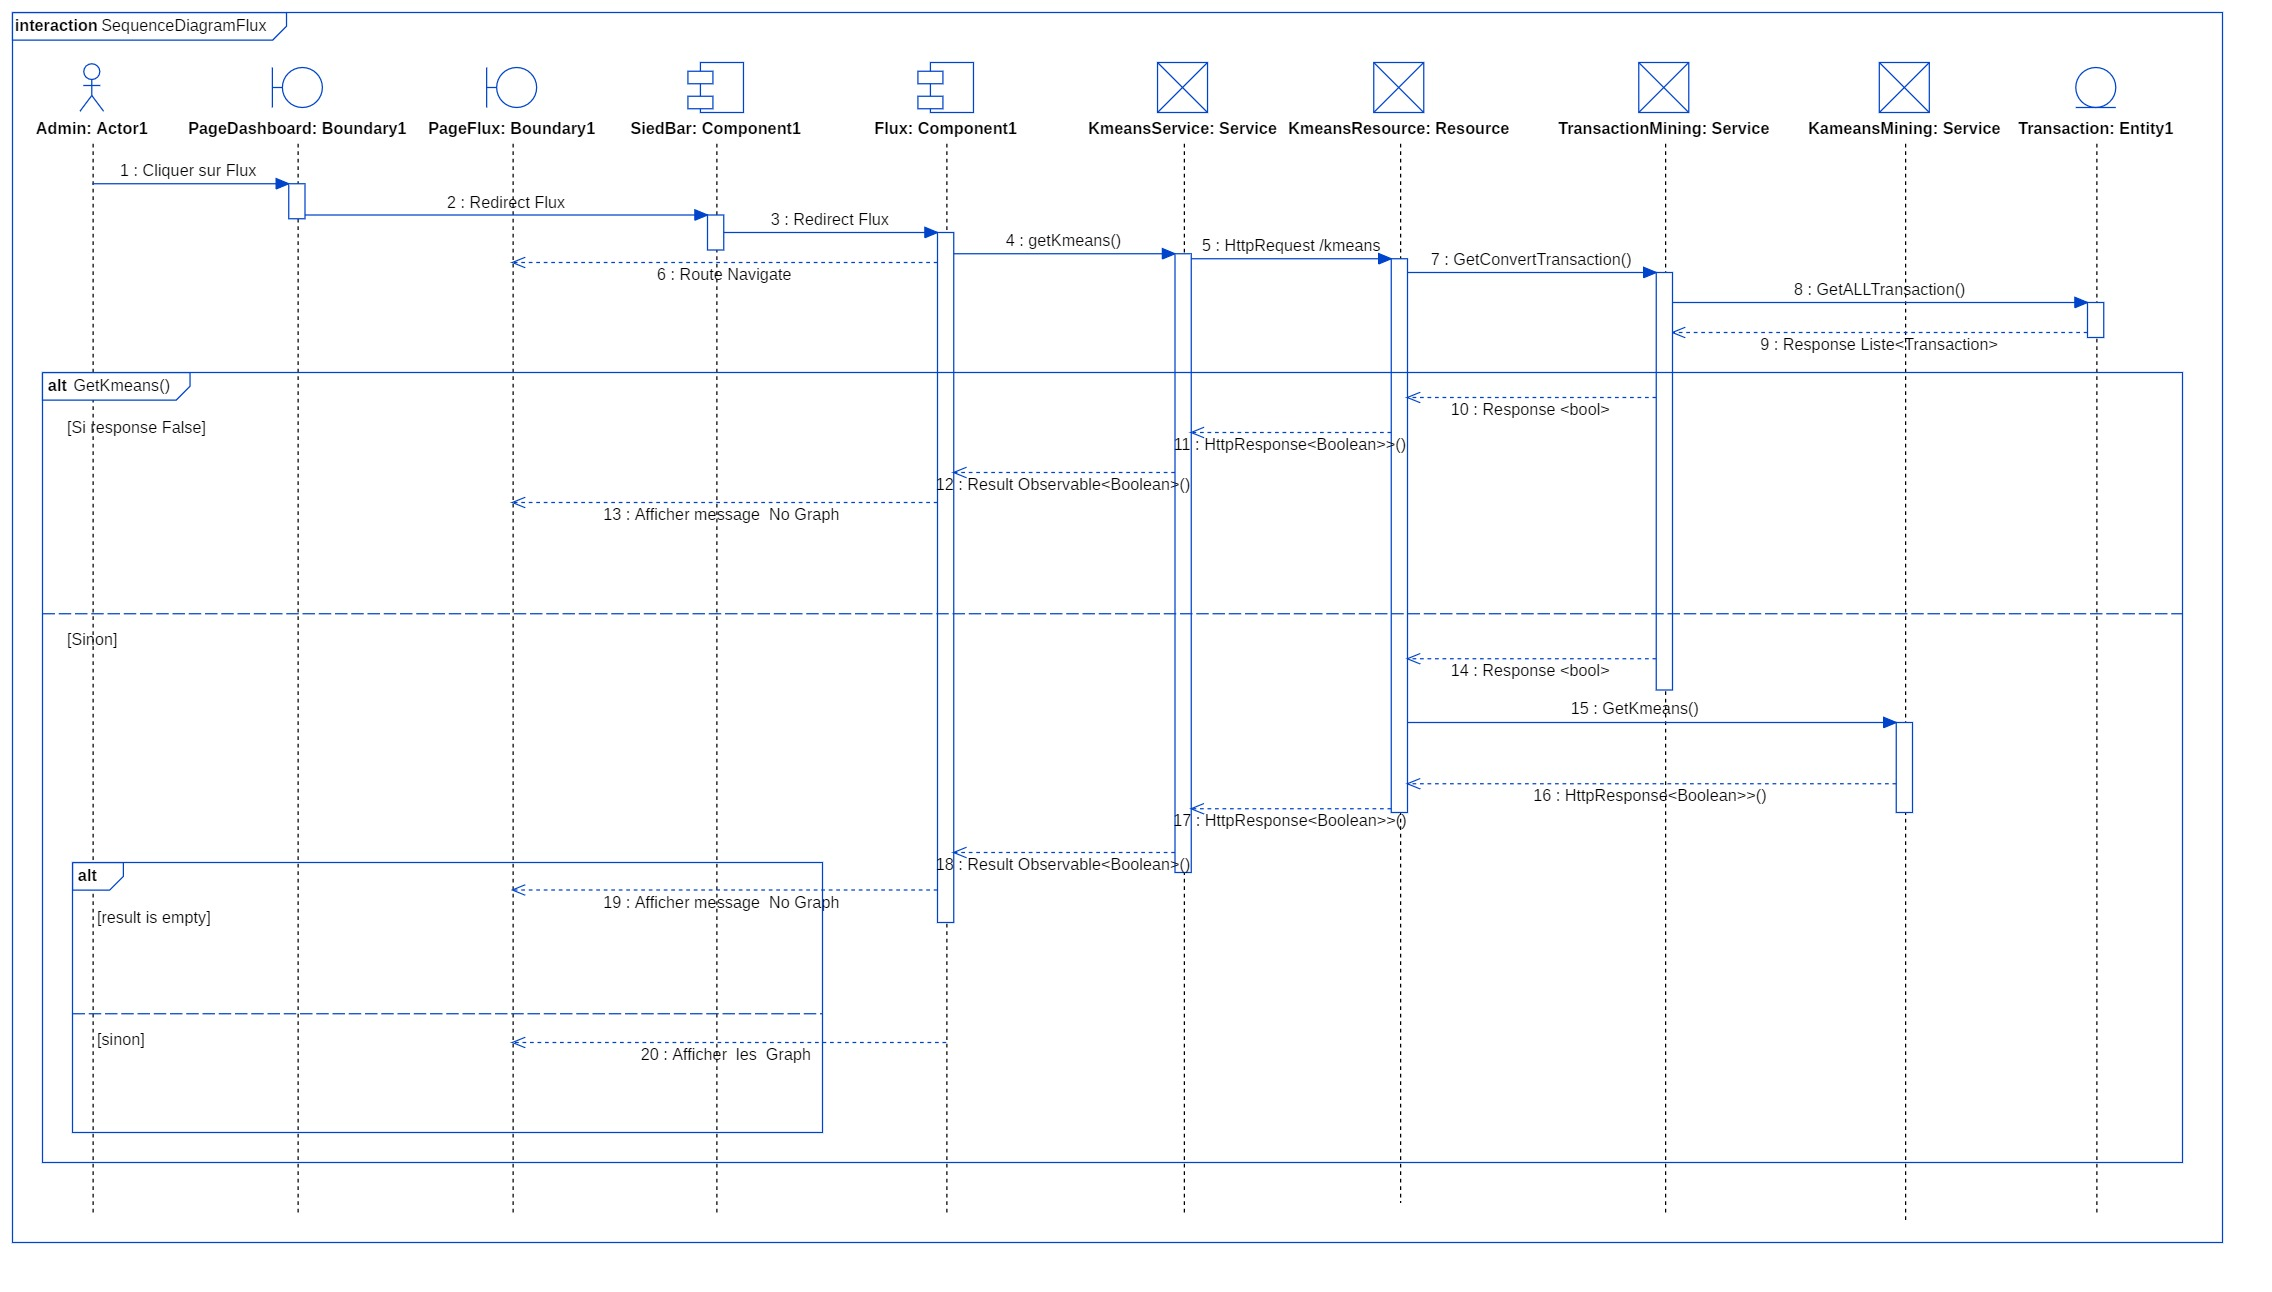
\includegraphics[width=1.4\columnwidth,angle=90]{chapitres/chapitre7/figures/SequenceDiagramFlux.jpg}
\caption{Diagramme de séquence du cas d'utilisation "Consulter les fluxe"}
\label{fig:SequenceDiagramFlux}
\end{figure}
\section{Réalisation}
L'interface illustrée dans la figure \ref{fig:flux1} permet d'afficher la premières partie
 des graphiques qui présentent le résultat des analyses de flux. 

\begin{figure}[!ht]\centering
\fbox{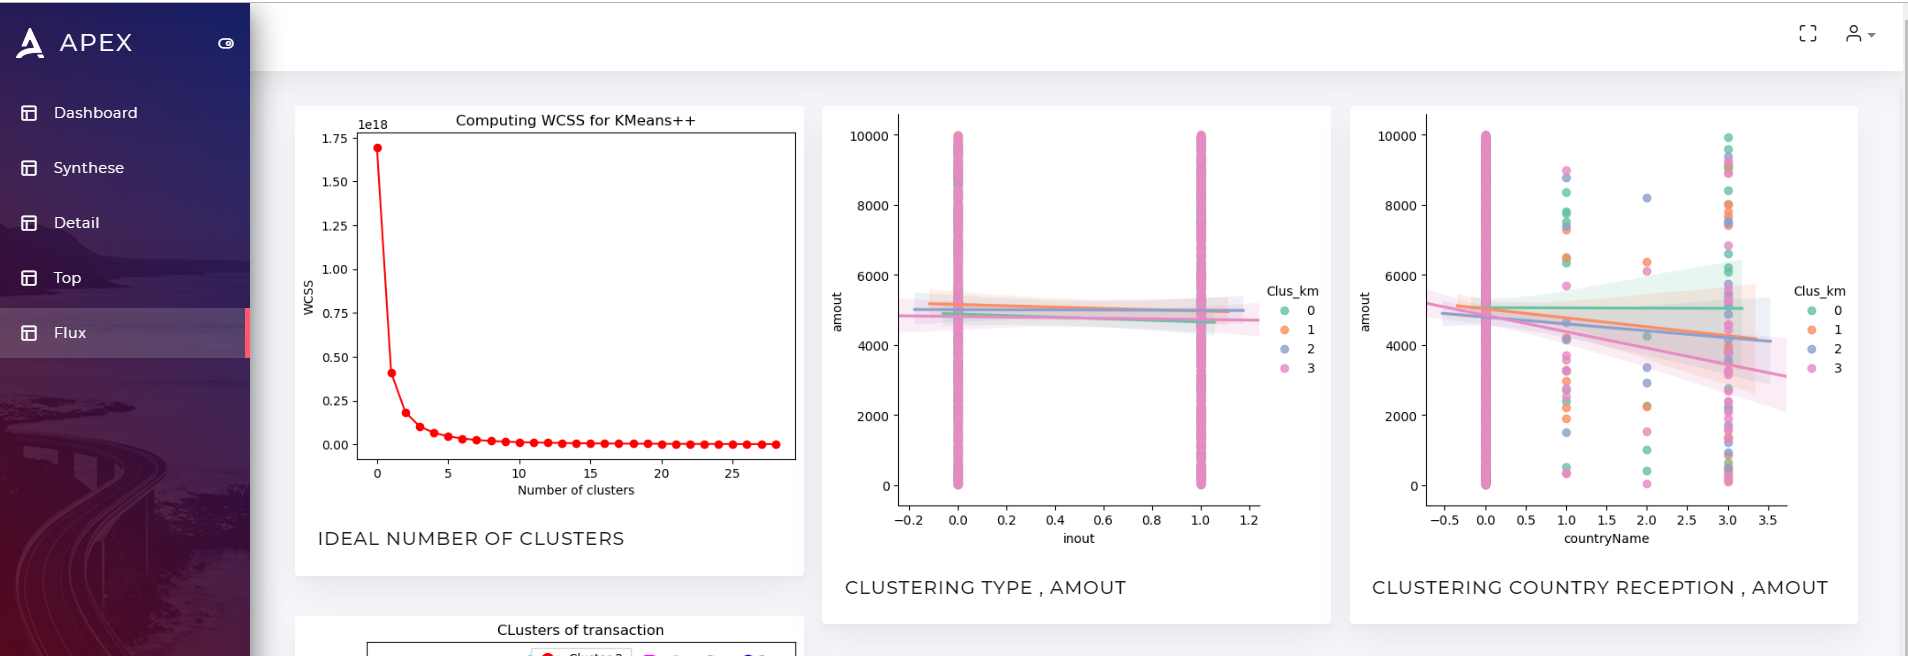
\includegraphics[width=1\textwidth]{chapitres/chapitre7/figures/flux1.PNG}}
\caption{Interface consulter les flux}
\label{fig:flux1}
\end{figure} 
L'interface illustrée dans la figures \ref{fig:flux1} permet d'afficher la deuxième partie   
 des graphiques qui présentent le résultat des analyses de flux.  
\begin{figure}[!ht]\centering
\fbox{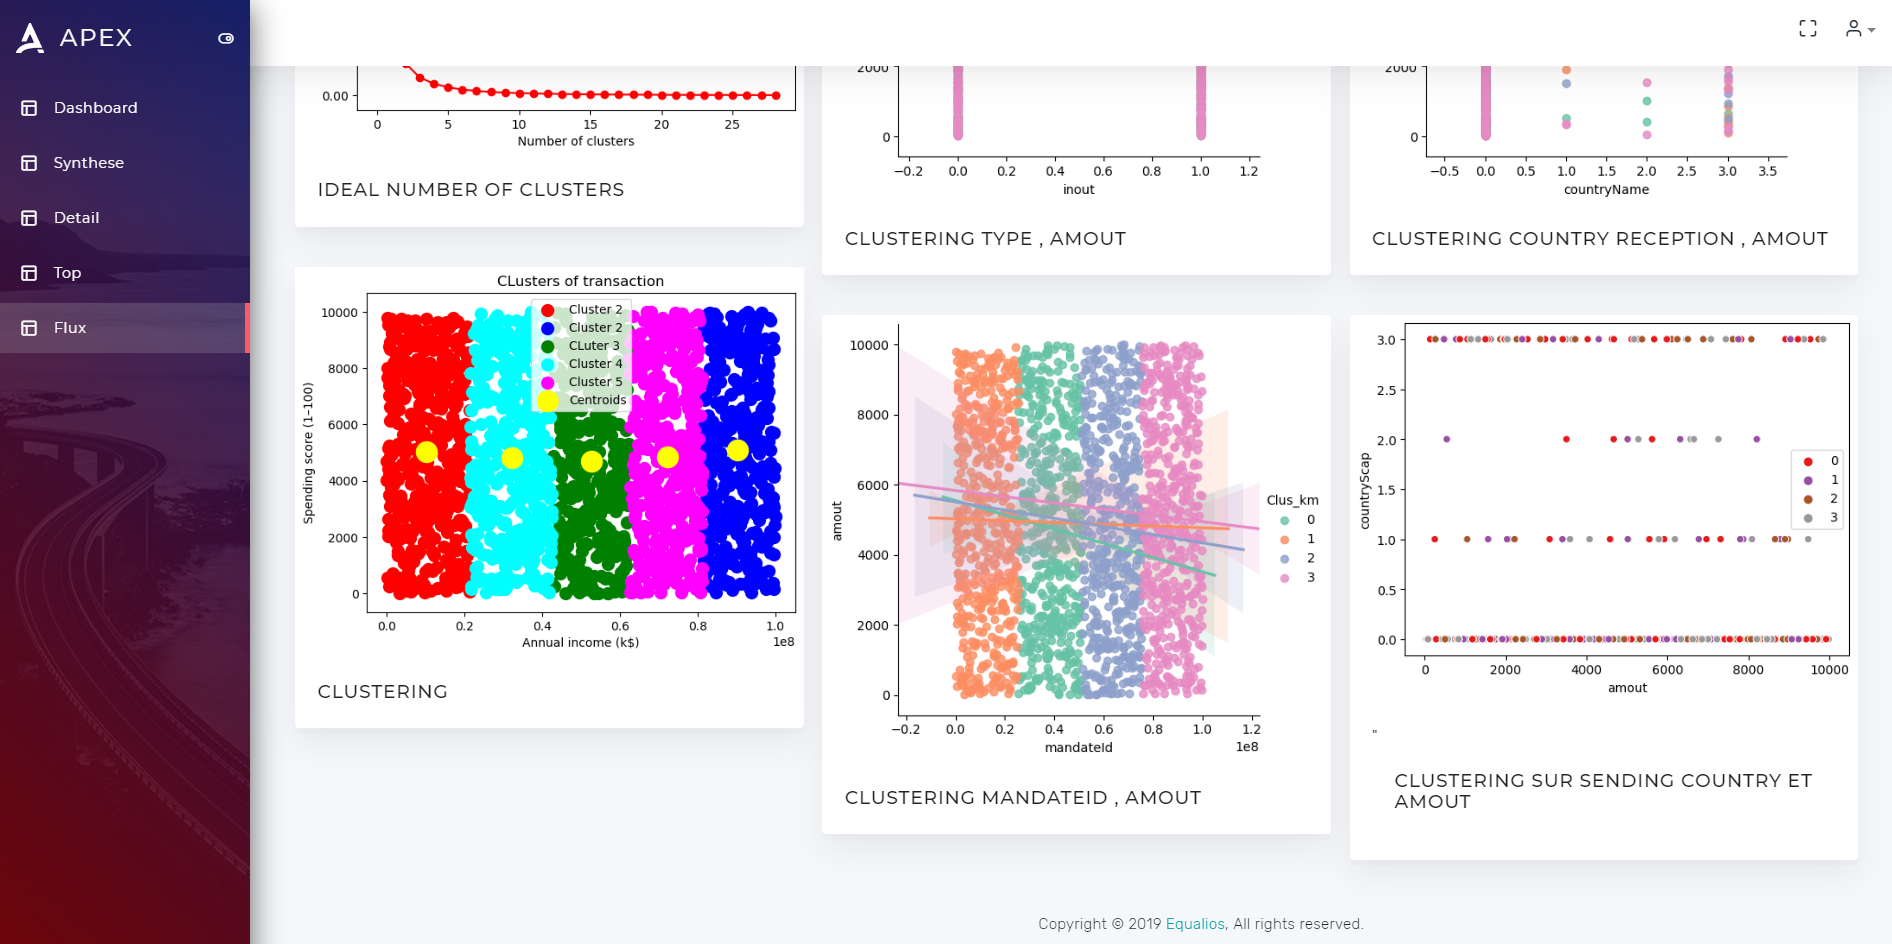
\includegraphics[width=1\textwidth]{chapitres/chapitre7/figures/flux2.PNG}}
\caption{Interface consulter les flux}
\label{fig:flux2}
\end{figure} 
\section{Environnement de travail}
Dans ce chapitre nous avons découvert une autre vision, d'autres technologies, langages et logiciels.
\subsection{Environnement logiciel}
\subsubsection*{PyCharm }
PyCharm est un environnement de développement intégré utilisé pour programmer en Python,  d\'evelopp\'e par l'entreprise JetBrains .
\begin{figure}[!ht]\centering

\includegraphics[width=0.2\textwidth]{chapitres/chapitre7/figures/pycharme.png}
\caption{Pycharm logo}
\label{fig:pycharme}
\end{figure}
\subsubsection*{Jupyter Notebook }
Jupyter Notebook est une application web utilisée pour programmer dans plus de 40 langages de programmation, dont Python, Julia, Ruby, R, ou encore Scala2. Jupyter est une évolution du projet IPython. Jupyter permet de réaliser des calepins ou notebooks, c'est-à-dire des programmes contenant à la fois du texte en markdown et du code en Julia, Python, R... Ces notebooks sont utilisés en science des données pour explorer et analyser des données.
\begin{figure}[!ht]\centering

\includegraphics[width=0.2\textwidth]{chapitres/chapitre7/figures/Jupyter.png}
\caption{Jupyter logo}
\label{fig:Jupyter}
\end{figure}
\subsection{Argumentation des choix techniques}
\subsubsection*{Python}
Python est un langage de programmation interprété, orienté objet et de haut niveau avec une sémantique dynamique. Ses structures de données intégrées de haut niveau, combinées à un typage dynamique et à une liaison dynamique, le rendent très attrayant pour le développement rapide d'applications, ainsi que pour son utilisation en tant que langage de script ou de collage pour connecter des composants existants. La syntaxe simple et facile à apprendre de Python met l'accent sur la lisibilité et réduit donc le coût de la maintenance du programme. Python prend en charge les modules et les packages, ce qui encourage la modularité du programme et la réutilisation du code. L'interpréteur Python et la vaste bibliothèque standard sont disponibles gratuitement sous forme binaire ou source pour toutes les principales plates-formes et peuvent être distribués librement.
\begin{figure}[!ht]\centering

\includegraphics[width=0.4\textwidth]{chapitres/chapitrex/figures/python.png}
\caption{Python logo }
\label{fig:python}
\end{figure}
\subsubsection*{Flask}
Flask est un micro-framework web écrit en Python. Il s’agit d’un microframework car il ne nécessite ni outils ni bibliothèques particuliers. ... Cependant, Flask prend en charge des extensions pouvant ajouter des fonctionnalités d'application comme si elles étaient implémentées dans Flask même.
\begin{figure}[!ht]\centering
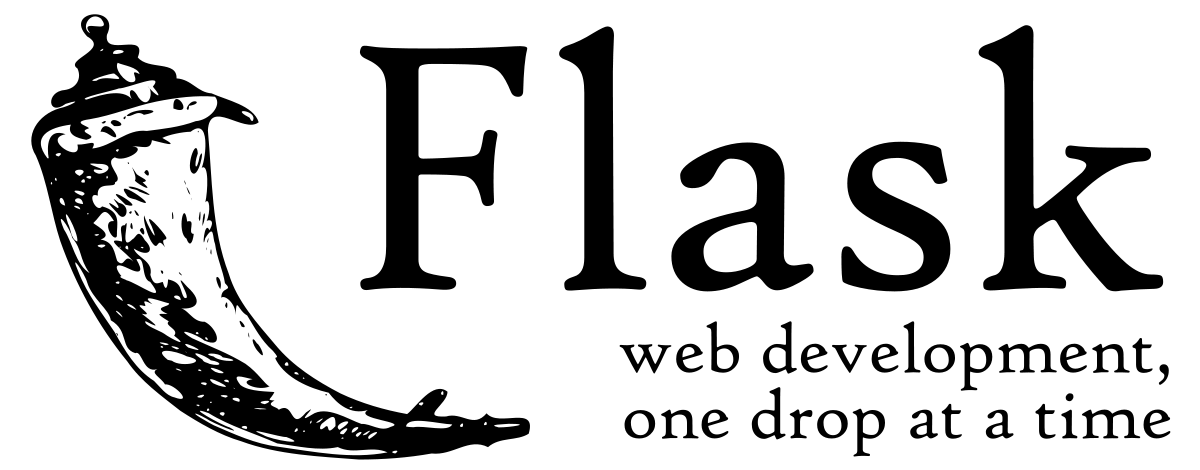
\includegraphics[width=0.4\textwidth]{chapitres/chapitre7/figures/flask.png}
\caption{Flask logo }
\label{fig:flask}
\end{figure}


\subsubsection*{Clustering K-means}

Le clustering K-means est l'un des algorithmes d'apprentissage automatique non supervisés les plus simples et les plus répandus.
En règle générale, les algorithmes non supervisés font des inférences à partir d'ensembles de données en utilisant uniquement des vecteurs d'entrée sans faire référence à des résultats connus ou étiquetés.
AndreyBu, qui a plus de 5 ans d'expérience en apprentissage automatique et enseigne actuellement ses compétences aux gens, déclare que «l'objectif de K-means est simple: regrouper des points de données similaires et découvrir les modèles sous-jacents. Pour atteindre cet objectif, K-means cherche un nombre fixe (k) de grappes dans un jeu de données. "
\begin{figure}[!ht]\centering
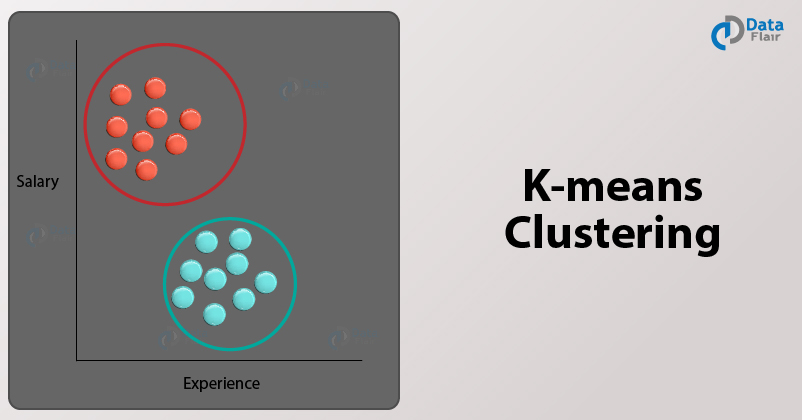
\includegraphics[width=0.4\textwidth]{chapitres/chapitre7/figures/KmeansClustering.jpg}
\caption{KmeansClustering }
\label{fig:KmeansClustering}
\end{figure}
\subsubsection*{Matplotlib}
Matplotlib a vu le jour pour permettre de générer directement des graphiques à partir de Python. Au fil des années, Matplotlib est devenu une librairie puissante, compatible avec beaucoup de plateformes, et capable de générer des graphiques dans beaucoup de formats différents.
\begin{figure}[!ht]\centering
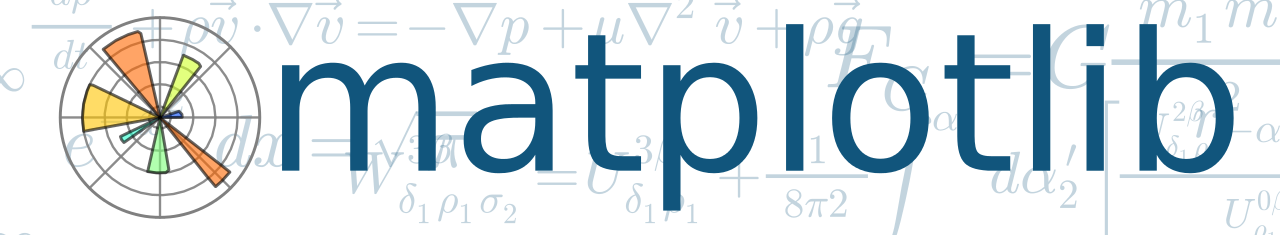
\includegraphics[width=0.4\textwidth]{chapitres/chapitre7/figures/Matplotlib.png}
\caption{Matplotlib logo }
\label{fig:matplotlib}
\end{figure}
\subsubsection*{Pandas}
Pandas est une bibliothèque écrite pour le langage de programmation Python permettant la manipulation et l'analyse des données. Elle propose en particulier des structures de données et des opérations de manipulation de tableaux numériques et de séries temporelles. Pandas est un logiciel libre sous licence BSD.
\newpage
\begin{figure}[!ht]\centering

\includegraphics[width=0.4\textwidth]{chapitres/chapitre7/figures/pandas.jpg}
\caption{Pandas logo }
\label{fig:pandas}
\end{figure}
\subsubsection*{Faker}
faker fait partie de ses libs que j’ai toujours voulu écrire sans jamais prendre le temps de le faire. Comme arrow par exemple. Et puis un jour quelqu’un le fait, et je suis à la fois soulagé de ne pas avoir tenté de le faire (au risque de ne pas réussir aussi bien) et un peu déçu d’être passé à côté de la bonne idée.

Le principe de la lib est très simple : générer des données bidons. Noms, numéros de téléphone, adresses physiques ou email… C’est utile pour tout un tas de choses :
\begin{enumerate}[label=$\bullet$]

    \item Faire des tests, évidement.
\item Créer des bots, des crawlers et tout autre programme qui doit se faire passer pour un utilisateur.
\item Remplir une base de données vide en attendant que les utilisateurs réels remplissent le site. Cela évite le sentiment d’arriver sur un service désert. Tous les sites de rencontre font ça.
\item Générer un contexte artificiel, par exemple pour un jeu vidéo.
\end{enumerate}
\begin{figure}[!ht]\centering

\includegraphics[width=0.4\textwidth]{chapitres/chapitre7/figures/faker.png}
\caption{Faker logo }
\label{fig:faker}
\end{figure}
\section*{Conclusion}
Lors de ce chapitre, nous avons r\'ealis\'e une petite expérimentation analysant des flux de transactions afin d'avoir une vision globale de notre base de données et de nous préparer pour passer à d'autres missions.
